\documentclass{article}
\usepackage[utf8]{inputenc}
\usepackage{graphicx}
\usepackage{amsmath}
\usepackage{hyperref}
\usepackage[a4paper, textwidth=450pt]{geometry}

\graphicspath{ {./data/} }

\title{EP4 Homework 4}
\author{Adam Kit}
\date{4 May 2020}


\begin{document}

\maketitle

\section{Task 1}
An electron performs underdamped, but nearly harmonic, oscillations with a frequency of 1015 Hz.  After which time period it will loose 90 percent of its initial energy $E_0$.
\subsection*{Lorentz Oscillator }

\subsection{Task 2}
Find the average scattering angle $\bar{\theta} $ resulting for the Thomson model of atom.  Use the fact that the scattering angles are small.
\subsection*{Plum Model}

Thomson suggested that the electrons were distributed in a positively charged medium, thus he shot a material of atoms with lots of high-energy $\alpha-$particles and watched how they $\alpha$-particles scattered. If the particle were to pass the atom, which has a radius $R$, at a distance $b$(collision parameter) from the center of the atom, we would see one of two different scenarios, depending on b.
For the scenario of $b > R$: since the atom is neutral, the $\alpha$-particle's trajectory is not affected.
For the scenario $b<R$: there is an electrostatic interaction and the particle is deviated by a small angle $\theta (b)$ which will lead to an intensity profile $I(\theta)$ of the particle beam hitting a capturing screen. This can also be modeled by a 2D random walk, where the intensity is described by N number of steps of $s$ step length, and $\bar s$ average step length: $$ I(s) \propto e^{-\frac{s^2}{N\bar s^2}}$$ or in terms of random angle deviations $\theta$ and average angle deviation $\bar \theta$:  $$I(\theta) \propto e^{-\frac{\theta ^2}{N \bar\theta ^2}} $$ I propose to first find $\bar s$ and from there determine $\bar \theta$ from the idea of
\section{Task 3}
Find how the distance $\Delta r$ between two adjacent electron orbits varies with increasing radius in the limit of large quantum numbers n.
\subsection*{Electron Radius}
In the Figure \ref{radiustrans} we see the relationship between the distance between adjacent electron orbits. This comes from the Bohr relationship of electron orbit radius $r_n = a_0 \frac{n^2}{Z}$ where $a_0 = 0.0529*10^{-9}$m is the Bohr radius of the first electron orbit, and Z the atomic number of the atom in whose electrons are in question. We can then describe the distance between two adjacent orbits as: $$\Delta r = r_{n+1} - r_{n} = \frac{a_0}{Z}((n+1)^2 - n^2) = \frac{a_0}{Z}(2n +1)$$
Although linear, and seemingly increasing, note the size of $a_0$ and the division by Z. For the hydrogen atom (Z = 1) Even if $n =1*10^{11} $, we find that $\Delta r = 10.58$ meters. !

\begin{figure}
      \centering
      \caption{Linear relationship of the distance between adjacent electron orbits for atomic numbers Z: 1-8. Note: the y axis is scaled by $1*10^{-7}$}
      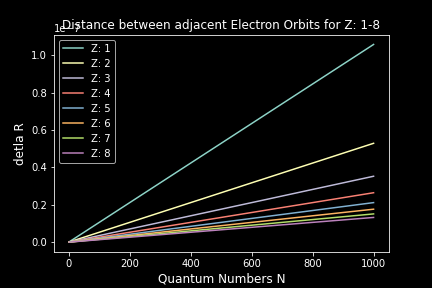
\includegraphics[scale = 0.8]{radiustrans.png}
      \label{radiustrans}

\end{figure}

\section{Task 4}
Show that the energy of the transitions between two adjacent orbit $\Delta E$ is proportional to $n^{-3}$ in the limit of large quantum numbers.
\subsection*{Transition Energies}
Just like for problem three, I have graphed the relationship between $\Delta E$ and n. The $n^{-3}$ proportion is apparent in Figure \ref{energytrans}. This comes from the energy an electron has in a given orbit n being $E_n = -E_0 \frac{Z^2}{n^2}$ and the relationship being:
$$\Delta E = E_{n+1} - E_n = -E_0 Z^2 [\frac{1}{(n+1)^2} - \frac{1}{n^2}] =  -E_0 Z^2 \frac{-2n -1}{n^3 + 2n^2 + n} \propto -E_0Z^2 n^{-3}$$ as for $n^3 >> n^2 >> n$ and the other terms will drop.

\begin{figure}
      \centering
      \caption{Relationship of the $\Delta E$ between adjacent electron orbits for atomic numbers Z: 1-8. Note the scaling is logarithmic, as these values are decreasing very very quickly as N is increasing, thus to properly show, I chose to plot logE instead}
      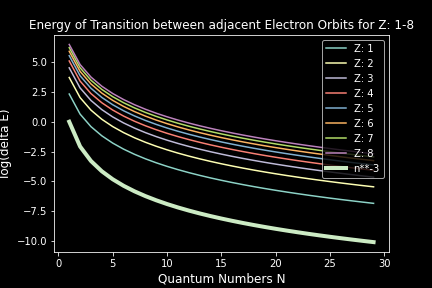
\includegraphics[scale = 0.8]{energytrans.png}
      \label{energytrans}

\end{figure}


\section{Task 5}
Which spectral lines will appear in the emission spectrum of an atomichydrogen gas upon irradiating it with ultraviolet light with the wave length of 100 nm?




\end{document}
